\documentclass{beamer}
\usepackage[utf8]{inputenc}
\usepackage{hyperref}

\usetheme{Madrid}
\setbeamertemplate{headline}{}
\setbeamertemplate{items}[circle]
\beamertemplatenavigationsymbolsempty

\title{Open Source}
\subtitle{Principles of Open Source}
\author{Florian Weingartshofer}
\institute{FH Hagenberg}
\date{\today}
\subject{English}

\begin{document}
\titlepage

\begin{frame}
  \frametitle{Outline}
  \tableofcontents
\end{frame}

\section{Definition}
\section{Usage}
\section{Tutorial}

\begin{frame}
  \frametitle{What's Open Source?}
  \begin{columns}
    \begin{column}{0.5\textwidth}
%      A way of developing Software
      \begin{center}
        \Large
        Transparency

        Collaboration

        Release early and often

        Meritocracy

        Community
      \end{center}
    \end{column}
    \begin{column}{0.5\textwidth}  %%<--- here
      \begin{center}
        \begin{figure}
          
\includegraphics[scale=0.03]{./img/open.jpg}
          \caption{unsplash.com/@stairhopper}
        \end{figure}
      \end{center}
    \end{column}
  \end{columns}
\end{frame}

\begin{frame}
  \frametitle{Who's Using It?}
  \begin{columns}
    \begin{column}{0.5\textwidth}
      \begin{center}
        \begin{figure}
          
\includegraphics[scale=0.06]{./img/tux.png}
          \caption{Tux}
        \end{figure}
      \end{center}
    \end{column}
    \begin{column}{0.4\textwidth}
      \begin{block}{Everybody Is Using OS!}
        
        Web-Dev
        
        Programming Languages

        Protocols
      \end{block}
      \begin{exampleblock}{Many are Contributing!}
        \begin{enumerate}
        \item Microsoft
        \item Google
        \item Red Hat
        \item IBM
        \end{enumerate}
        
      \end{exampleblock}
    \end{column}
  \end{columns}
\end{frame}

\begin{frame}
  \frametitle{Open Source Crash Course}
  \begin{columns}
    \begin{column}{0.4\textwidth}
      \Large
      Source Hosting

      Add a License: \href{https://choosealicense.com/}
      {choosealicense.com}

      Upload Files

      Thats it!
    \end{column}
    \begin{column}{0.3\textwidth}
      \begin{block}{Source Hosting}
        GitHub.com

        GitLab.com

        BitBucket.org
      \end{block}      
      \begin{block}{Licenses}
        MIT

        GPLv2.0 or GPLv3.0

        BSD

        CC-BY-4.0
      \end{block}      
    \end{column}
  \end{columns}
  \begin{figure}
    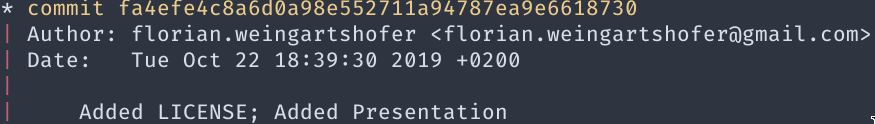
\includegraphics[scale=0.3]{./img/git.png}
      \caption{Git}
    \end{figure}
\end{frame}

\begin{frame}
  \frametitle{Free Software}
  \begin{columns}
    \begin{column}{0.6\textwidth}
      \begin{figure}
        
\includegraphics[scale=0.3]{./img/gnu_penguin.png}
        \caption
          {GNU and Penguin; Free Arts License}
      \end{figure}
    \end{column}
    \begin{column}{0.4\textwidth}
      \Large
      Political

      Hard Liner

      Stricter Criteria
    \end{column}
  \end{columns}
\end{frame}


\begin{frame}
  \frametitle{Questions?}
  \begin{center}
    \begin{figure}
      
\includegraphics[scale=0.3]{./img/tux_questions.png}
    \end{figure}
    The Presentation is obviously Open Source at
    \underline{
      \href{https://github.com/flohero/opensource-presentation}
           {github.com/flohero/opensource-presentation}
    }
    \end{center}
\end{frame}

\begin{frame}
  \frametitle{Sources}
  \begin{center}
    \Large
    \href{https://opensource.com/open-source-way}{opensource.com}
    
    \href{https://twitter.com/filmaj}{twitter.com/filmaj}

    \href{https://en.wikipedia.org}{wikipedia.org}

    \href{https://github.com}{github.com}
    
  \end{center}
\end{frame}
\end{document}
